
\section{Why Photovoltaic}

	\paragraph{Abundance}
	The total solar irradiance hitting the outer Earth atmosphere is around \SI{1361}{\watt\per\square\metre},\cite{Kopp2011} which, considering our planet cross section area, makes \SI{1.6e17}{\watt}.
	Nature conveys this energy in plenty of ways, including the generation of every renewable and most of non-renewable energy sources.
	Solar energy is effectively the primary energy source for our planet's ecosystem, so it is the most interesting source of energy for human usage.

%	JUST A SMALL PART OF THIS INCOMING ENERGY IS GETTING USED


	\paragraph{Availability}
	The ubiquitous availability of solar power can be the leverage for an economical power levelling across different regions of the planet.
	Indeed, the abundance of solar irradiation (represented in \cref{fig:world_map-PVOUT} by the ratio between the photovoltaic electric energy that can be obtained over the nominal power of an installed solar panel) is quite high in most of the regions where life quality is seriously affected by economical situation (represented in \cref{fig:world_map-HDI} by the Human Development Index).

	\begin{figure}%[!hbtp]%
		\makebox[\textwidth][c]{
			\parbox{1.1\textwidth}{
				\centering
				\begin{subfigure}[b]{1\textwidth}
					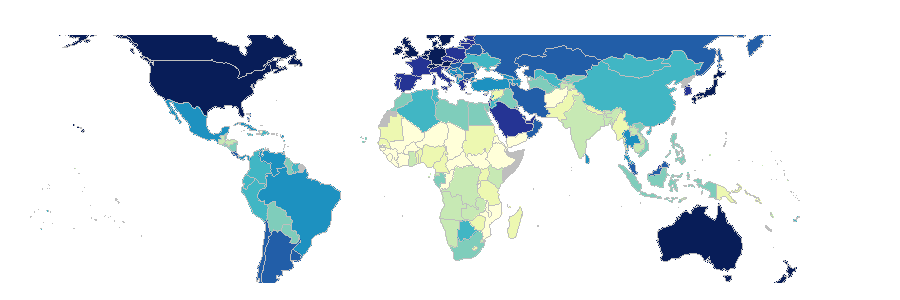
\includegraphics[width=0.9\textwidth]{world_map-HDI/world_map-HDI.pdf}
					\subcaption{Human development index by region}\label{fig:world_map-HDI}
				\end{subfigure}

				\begin{subfigure}[b]{1\textwidth}
					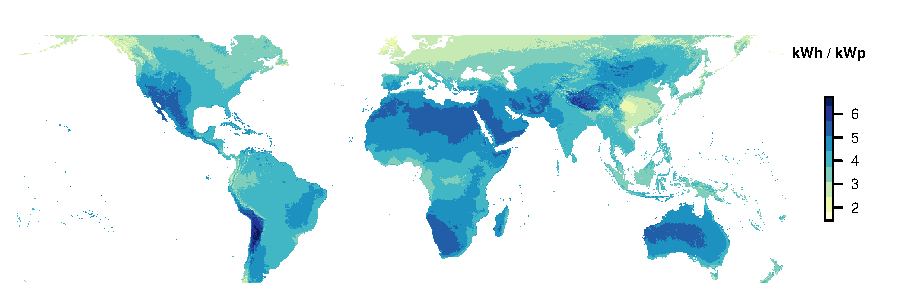
\includegraphics[width=0.9\textwidth]{world_map-PVOUT/world_map-PVOUT.pdf}
					\subcaption{Daily photovoltaic electricity potential}\label{fig:world_map-PVOUT}
				\end{subfigure}

				\begin{subfigure}[b]{1\textwidth}
					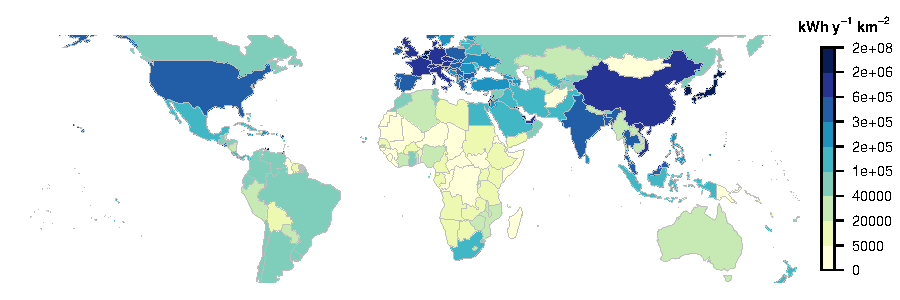
\includegraphics[width=0.9\textwidth]{world_map-electrical_vs_land/world_map-electrical_vs_land.pdf}
					\subcaption{Yearly electricity consumption over region land area}\label{fig:world_map-electrical_vs_land}
				\end{subfigure}
				\mycaption[Geographical distribution of development, sunlight and consumption.]{Data in (\textbf{a}) represent the human development index:
					"a summary measure of average achievement in key dimensions of human development: a long and healthy life, being knowledgeable and have a decent standard of living"
					from UNDP\cite{UNDP2018} (missing data in grey); data in (\textbf{b}) represents the photovoltaic electricity potential: considering a photovoltaic module installed in a region, is the ratio between the average daily produced energy, in kWh, and the nominal power, or nameplate capacity, of the installed module;\cite{Solargis2018} data in (\textbf{c}) represents the yearly electricity consumption\cite{CIAa} (comparing total electricity generated annually plus imports and minus exports) on a country scale divided by country land surface,\cite{CIA} expressed in kilowatt-hour per year and per square kilometre.}\label{fig:world_map}
			}}
	\end{figure}

	\paragraph{Resilience}
	The usage of photovoltaic energy source is compatible with a distributed and decentralized network model.
	Such a power network can be much more resilient than the fossil fuels based system, with the only single-point-of-failure being the climate variability.
	%	is the electric energy production method that best matches a distributed and decentralized network model, 
	Combined with accumulation (needed for night time usage) and with other energy sources, it can be the pivot of an extremely reliable electric energy provisioning system.

	\paragraph{More energy is not enough} It is intuitive that increasing the energy production is a high-price solution to the growing energetic demand.
	Indeed, in some regions a decrease in the electricity consumption has to be included for a long-term solution.
	For example, a study\cite{Margolis2016} reports that if every rooftop (not considering utility-scale solar facilities) in United States of America was covered with solar panel, just the 39~\% of its nowadays national consumption would be covered.
	In \cref{fig:world_map-electrical_vs_land} we can see how electricity consumption density is greatly inhomogeneous and comparing with the photovoltaic potential map in \cref{fig:world_map-PVOUT}, it is evident that such a problem is shared with many other poorly insulated but energy eager regions.
	Both an increase in machinery's efficiency and a change in life-style can be part of the solution, following the example and thinking at life-style, in USA the \textsl{per capita} energy usage is more than twice the European average, and five times the Latin America average.\cite{IEA}

	\paragraph{And more research is needed} Every source of electrical energy we can think of works \textsl{via} the conversion of motive power (a flow of steam, wind, or water, waves, tides...) to electricity, which relays on the well established electric generator.
	Except photovoltaic energy.
	This very simple difference already hints for the huge conceptual and technological step required by photovoltaics as compared to other electrical energy sources.

	% transducer
	\mysection[Relevant Physics]{Relevant Physics for Stacked Semiconductor Thin Films}

	\subsection{Energy Levels and Occupancy}
			
	\begin{SCfigure}
		\centering
		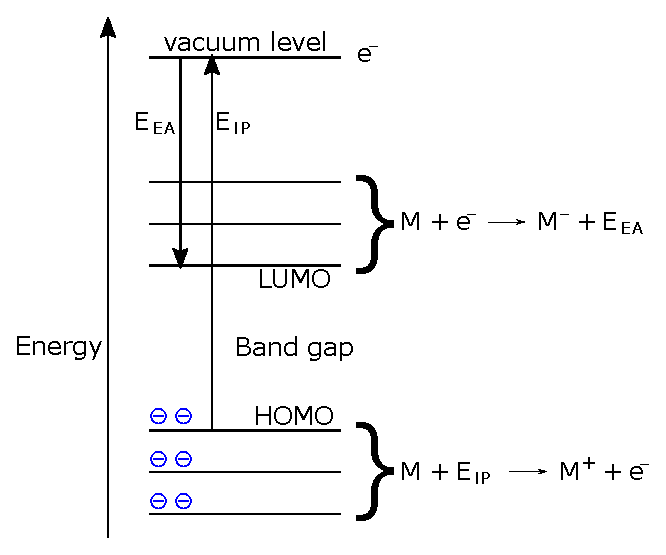
\includegraphics[width=0.7\textwidth]{homo_lumo/homo_lumo.pdf}
		\mycaption[Representation of HOMO and LUMO levels.]{
			Each horizontal line represents the energy of a molecular orbital in a neutral molecule at ground state.
			So the bottom group are the occupied orbitals while the upper group are the virtual ones.
		}\label{fig:homo_lumo}
	\end{SCfigure}
		
		\paragraph{HOMO and LUMO}
		The energy that an electron can have when it is bound in a nanometric volume (like a molecular bond) is quantized, the possible energies are represented in \cref{fig:homo_lumo}.
		The lowest levels represent the ones filled with electrons and their energy is defined as the energy that can be provided to a neutral isolated molecule at its ground state which result in one electron being separated from it at an infinite distance.
		The minimum of these ionization energies, is the \gls{homo}.
		The highest levels are virtual ones and represent the energies that can be gained when an unbound electron gets bound to a isolated molecule which was neutral and at its ground state.
		The maximum of these electron affinity energies, is the \gls{lumo}.
		The difference between \gls{homo} and \gls{lumo} is named band gap.
		After these processes, the molecule will geometrically change and release some reorganization energy, but this is not included in the \gls{homo} and \gls{lumo} definition (\textsl{i.e.} a vertical transition is considered).

		\paragraph{Valence and conduction bands in crystalline solids}
		As we saw, for an isolated molecule the energy levels are discrete values.
		On the contrary, for materials where electrons are delocalized in a periodic potential (\textsl{e.g.} in a crystal structure) we have continuous bands (ranges) of allowed electronic energies separated by energy gaps \cite{WikipediaPeriodic}.
		For a 3D crystal, the density of states can be approximated to be the \gls{dos} of a free electrons gas where it grows with the square root of the energy, as represented in \cref{fig:DOS} \cite[140]{Kittel2004}.
		
		\paragraph{Valence and conduction bands in amorphous solids}
		In amorphous solids, the allowed electronic energy is still composed by bands but localised states can appear inside the band gaps and the band edges are less defined.
		These tails of the edges are usually localised states whose mobility is low, for this reason in amorphous solids the mobility gap is wider than just the band edges separation \cite[213]{Stenzel2005}.
%		The carriers close to the band edges (in the bottom of conduction band or in the top of the valence band) are typically localised and have
		
		\begin{SCfigure}
			\centering
			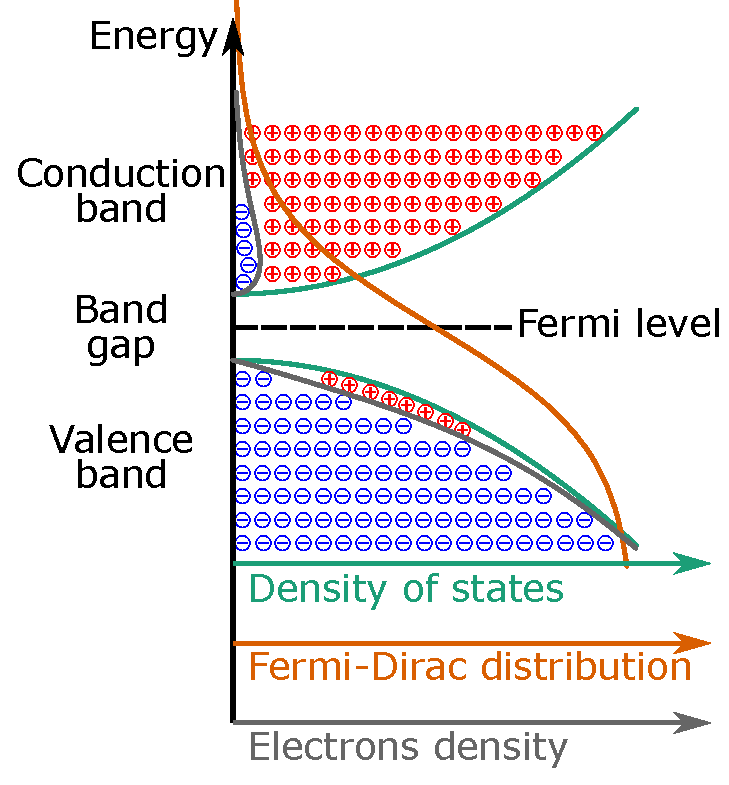
\includegraphics[width=0.6\textwidth]{DOS/DOS.pdf}
			\mycaption[Schematic representation of the density of states, Fermi-Dirac distribution, and electronic population for a crystalline intrinsic semiconductor.]{
				The green line indicates the density of states in a 3D crystalline solid, the two bands have been drawn with the same shape for simplicity, in general this could not be the case.
				The orange line is the Fermi\hyp{}Dirac distribution for the electrons population.
				The grey line is (approximatively) the product of the two aforementioned lines representing the electronic density energy distribution.
				
			}\label{fig:DOS}
		\end{SCfigure}
		

		\paragraph{Boltzmann and Fermi-Dirac statistics}
		For a system with defined temperature and total energy but various possible states at different energies, Boltzmann distribution gives the probability of finding it in a specific state.
		For example, considering electrons as non interacting particles we can estimate the conduction band population with:
		\begin{equation}\label{eq:boltzmann}
			n_|CB| = n_|DOS|\exp[\frac{q(\bar\mu-E_|CB|)}{k_|B|T}]
		\end{equation}
		where $n_|DOS|$ is the density of states representing the energy state degeneracy, $q$ is the elementary charge, $\bar\mu$ is the electrons electrochemical potential (quasi-Fermi level energy of electrons including the electrostatic contribution), and $E_|CB|$ is the conduction band energy including the local electrostatic potential.
		For low temperature or high electron density cases, the interactions between particles cannot be ignored.
		The inclusion of Pauli exclusion principle for fermions modifies the Boltzmann distribution into the Fermi\hyp{}Dirac distribution, which has not been used for the simulations performed in this thesis:
		\begin{equation}\label{eq:fermidirac}
		n_|CB| = \frac{n_|eDOS|}{\exp[q(E_|CB|-\bar\mu)/(k_|B|T)]+1}
		\end{equation}
		where $n_|DOS|$ has been replaced with the effective density of states $n_|eDOS|$ which considers the effective mass for interacting particles.

		\paragraph{Fermi level}
		Fermi level is an imaginary level (disregarding the actual states present in a system) defined for systems in thermodynamic equilibrium (no macroscopic particles or energy fluxes, neither internal nor from other systems) having an energy such that its occupancy probability is \SI{50}{\%}.
		For example, considering the 3D crystalline system represented in \cref{fig:DOS} if the Fermi level approaches the conduction band edge, the population at that edge state can be estimated using \cref{eq:fermidirac}: $\frac{n_|eDOS|}{\exp[q(E_|CB|-E_|CB|)/(k_|B|T)]+1} = n_|eDOS|/2$ so half full, while the valence band will be close to completely full (many electrons, very few holes).
		This level is ultimately the relevant potential for the charge carriers for a system in thermodynamic equilibrium, so if carriers can migrate through the system the Fermi level will have the same energy in every location of it.
		
		\paragraph{Doping}
		A perfect crystal semiconductor (no defects, no added dopants) is intrinsic, which means that its Fermi level is in the middle of the band gap and that the electron density in the conduction band is equal to the holes density in the valence band.
		In the example of the previous paragraph, where the Fermi level was close to the conduction band, the concentration of electrons greatly exceeds the holes density.
		This situation can happen in "extrinsic" or "doped" semiconductors, where the presence of, for example, positive ionic Schottky defects or oxidised species can compensate the charge of the high electrons concentration and result in a charge neutral material, as represented in \cref{fig:homojunction-doping}.
		It can also happen that the material, or a part of it, is just charged, for example due to the application of an electric field or in a space charge layer as will be seen further.
		
		\begin{SCfigure}
			\centering
			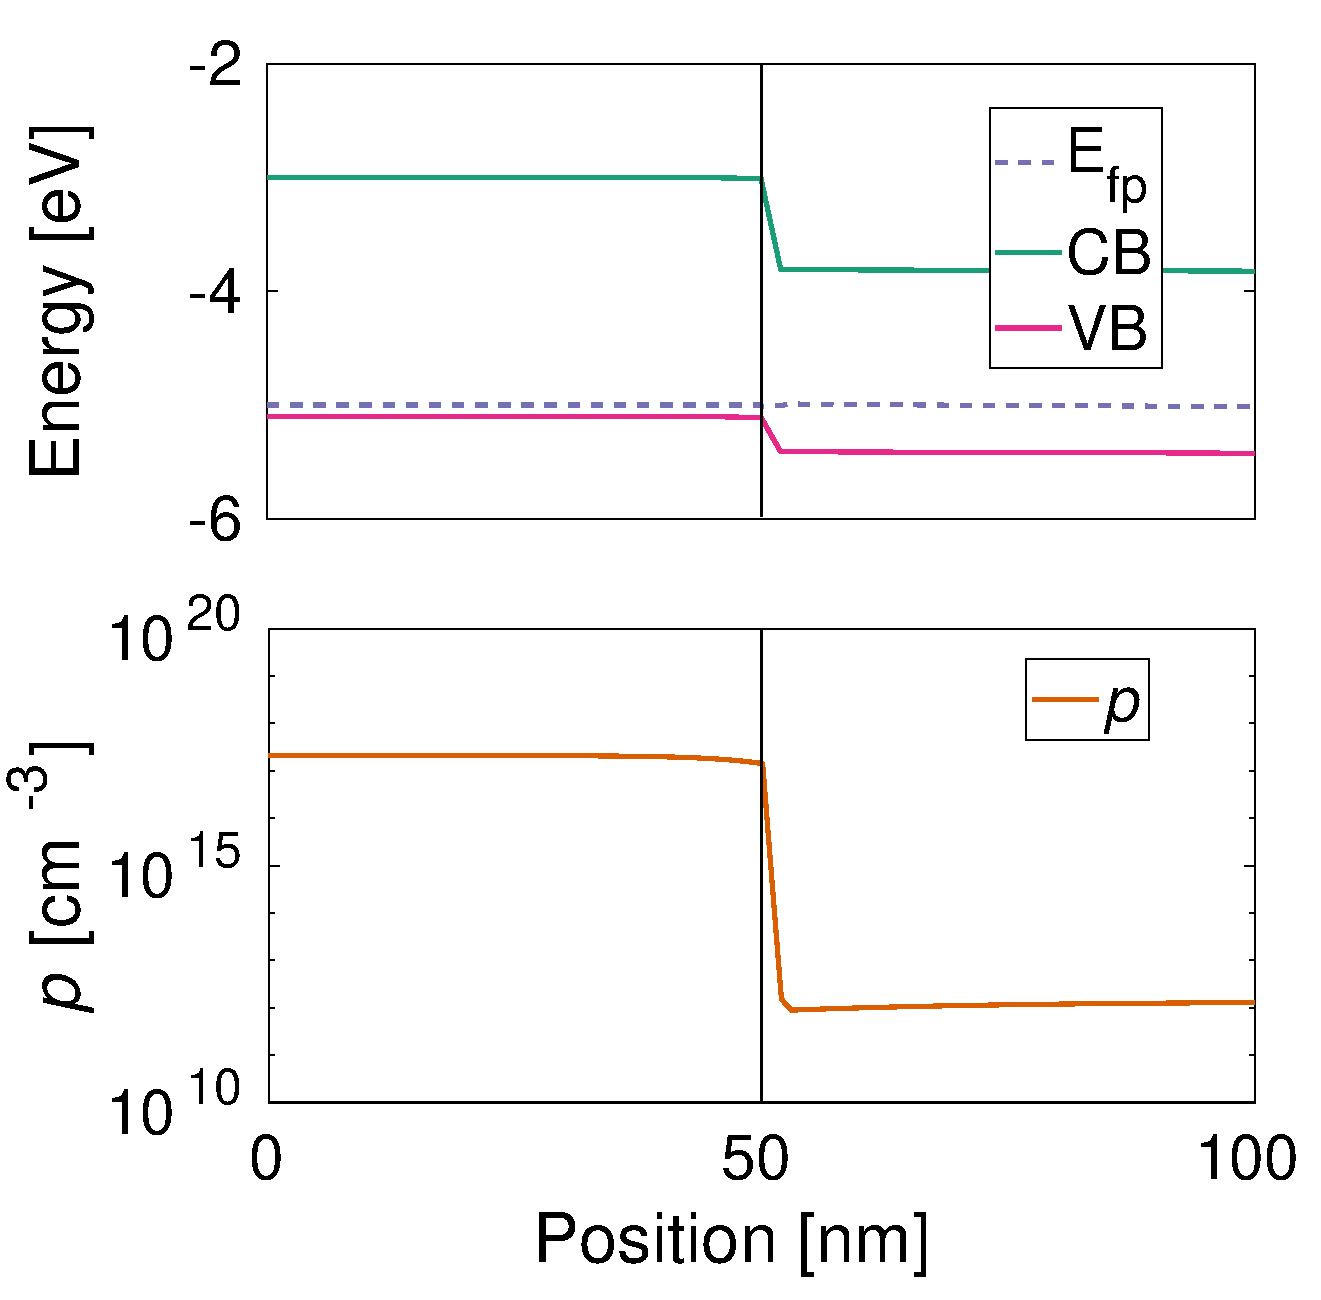
\includegraphics[width=0.5\textwidth]{holes_concentration/hj-holes_concentration.pdf}
			\mycaption[Representation of the relation between quasi\hyp{}Fermi level distance from respective band and carriers concentration.]{
				Simulation of an heterojunction.
				Notice how the $E_|fp|$ (valence band quasi\hyp{}Fermi level) distance from the valence band (top plot) relates to the holes concentration (bottom plot).}\label{fig:holes_concentration}
		\end{SCfigure}
	
		\paragraph{Quasi-Fermi level}
		For a system at steady state (or where the conditions are varying slowly enough to allow the carriers to thermalise within an energy band) but out of thermodynamic equilibrium the Fermi level is not defined any more.
		For example, if a constant illumination hits the system plenty of electrons will be promoted from the valence band to the conduction band and the occupancy described by \cref{eq:boltzmann} or \cref{eq:fermidirac} does not hold.
		In order to keep using the same convenient concepts, two quasi\hyp{}Fermi levels are introduced, where the electronic population in the conduction band and in the valence band are described separately, with two different electrons electrochemical potentials, as if they pertained to different systems in thermodynamic equilibrium.
		For simplicity, the quasi-Fermi level relative to the valence band is usually referred to the holes concentration rather than to the electrons.
		As the system is not in thermodynamic equilibrium, macroscopic particle currents can be present and this means that the energy of this level is location dependent, and can also be time dependent.
		Clearly, at thermodynamic equilibrium both the holes and the electrons quasi\hyp{}Fermi levels coalesce into the Fermi level.
		
		\paragraph{Quasi-Fermi level and occupancy}
		When observing a band diagram, like the one reported in \cref{fig:holes_concentration}, it is very easy to have an idea of the carriers concentrations observing the distance between the quasi\hyp{}Fermi levels and the band edges.
		For example, in \cref{fig:holes_concentration} we can see that the closer the $E_|fp|$ (quasi\hyp{}Fermi level relative to the valence band) gets to the valence band, the higher the holes concentration in it.
		
		\paragraph{Quasi\hyp{}Fermi levels and current}
		Coherently with the Fermi level concept, quasi-Fermi levels are the relevant potentials for the migration of holes in the valence band and electrons in the conduction band, treated separately.
		The quasi\hyp{}Fermi level considers both the internal chemical potential $\mu$ and the electrostatic potential $V_|E|$ and, as we will see below, these two quantities determine respectively the diffusion and the drift current.
		For this reason, a gradient in the valence or conduction band quasi\hyp{}Fermi level ($E_|fp|$ or $E_|fn|$) always indicates the presence of a current respectively of holes or electrons.
		
\subsection{Electrostatics}
Electrostatics refers to all electronic phenomena which does not intrinsically require a time varying quantity.


\begin{figure}
	\makebox[\textwidth][c]{
		\parbox{1.1\textwidth}{
			\centering
			\begin{subfigure}[t]{0.36\textwidth}
				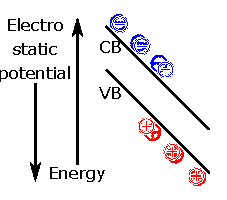
\includegraphics[scale=1.3]{drift_diffusion/drift_twobands.pdf}
				\subcaption{Drift due to electric field}\label{fig:drift_diffusion-drift}
			\end{subfigure}
			\qquad
			\begin{subfigure}[t]{0.66\textwidth}
				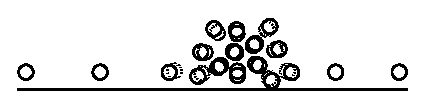
\includegraphics[scale=1.3]{drift_diffusion/diffusion-noncharged.pdf}
				\subcaption{Diffusion of particles}\label{fig:drift_diffusion-diffusion}
			\end{subfigure}
			\mycaption[Representation of drift and diffusion of charged particles.]{
				In (\textbf{a}) the drift of holes in the valence band and electrons in the conduction band due to an electric field is represented.
				In (\textbf{b}) the diffusion of generic particles due to differences in concentration is represented.
		}\label{fig:drift_diffusion}
		}
	}
\end{figure}

		\paragraph{Charged particles drift}\label{intro_drift}
		The electric field acts a Lorentz force on the charged particles.
		The movement of these particles due to the field is named "drift".
		The velocity is proportional to the electric field intensity and the mobility characteristic of the material and the type of charge.
		As represented in \cref{fig:drift_diffusion-drift}, in a typical energy diagram electrons drift downhill and holes drift uphill.

\paragraph{Particles diffusion}\label{intro_diffusion}
For all the non-fixed particles, part of the thermal energy is translational energy, regardless of their charge.
This means that the particles move in random directions, like in a Brownian motion for gases or in Drude model for classical description of electrons bouncing around.
The disordered motion statistically compensate differences in concentrations.
If the net diffusion flux is considered, this is proportional to the concentration gradient and to the diffusion coefficient (which is proportional to the mobility as described by Einstein relation).
As represented in \cref{fig:drift_diffusion-diffusion}, particles in highly concentrated zones tend to move towards less densely occupied ones.
Concentration of particles is the main contribution to the internal chemical potential $\mu$.

\begin{figure}
	\makebox[\textwidth][c]{
		\parbox{1.1\textwidth}{
			\centering
			\begin{subfigure}[t]{0.51\textwidth}
				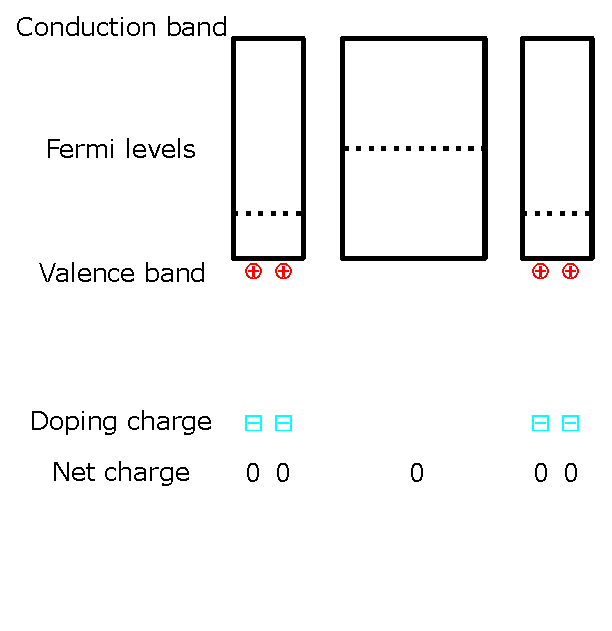
\includegraphics[scale=0.7]{homojunction/doping-ppipp.pdf}
				\subcaption{Homojunction before contact}\label{fig:homojunction-doping}
			\end{subfigure}
			\qquad
			\begin{subfigure}[t]{0.51\textwidth}
				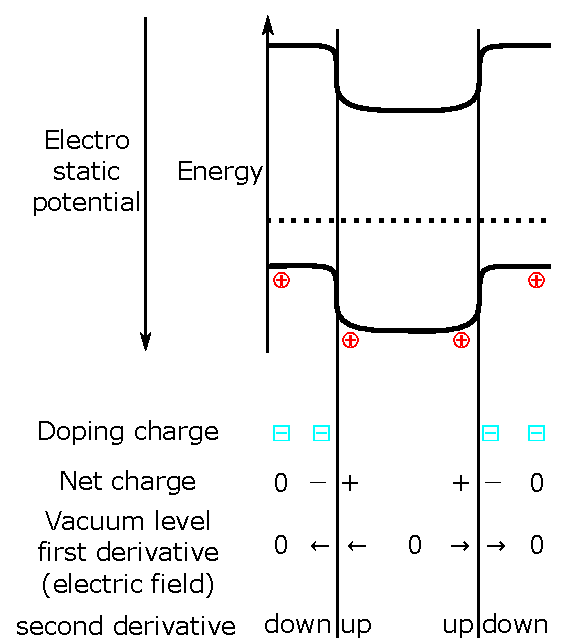
\includegraphics[scale=0.7]{homojunction/poisson_and_depletion-ppipp.pdf}
				\subcaption{After contact}\label{fig:homojunction-poisson_and_depletion}
			\end{subfigure}			
			\mycaption[Schematics of a p-i-p homojunction, with emphasis on depletion layers and representation of Poisson equation.]{
				In (\textbf{a}) three layers of the same material when doped to be respectively p-type, intrinsic (non doped), and p-type are represented.
				In order to compensate the fixed charges introduced by dopage and maintain the net charge neutrality, the p-type layers have the valence band rich in holes (clearly also the populations on the conduction band is affected by the doping, but not represented for simplicity).
				In (\textbf{b}) the three layers are brought in contact forming an homojunction.
				The holes flow through the interfaces following the Fermi level gradient, until it gets flattened.
				This generates space charge layers at the interfaces, where a net charge is present (the thickness of it is expected to be thicker in the intrinsic layer rather than in the doped ones, as described in \cpageref{intro-debye_length}).
				To easily understand the bending direction of the layers due to the net charge, the Poisson equation tells us that a positive charge means a positive vacuum level second derivative.
			}\label{fig:homojunction}
		}
	}
\end{figure}


		\paragraph{Poisson equation}
		The net charge in a location is related to the "curvature" (second derivative) of the electrostatic potential (\textsl{i.e.} the vacuum level) by the Poisson equation:
		\begin{equation}
			\nabla^2 V_|E| = -\frac{\rho}{\epsilon_0 \epsilon_|r|}
		\end{equation}
		where $V_|E|$ is the electrostatic potential (defined as the energy for adding a positive elementary charge), $\rho$ is the net charge obtained summing up all the charged particles concentrations in the location, and $\epsilon_0 \epsilon_|r|$ is the permittivity.
		For easing the understanding of the band diagram, the scheme in \cref{fig:homojunction-poisson_and_depletion} can be handful.
		As can be seen, in the zones where a net charge is present (space charge layers, depletion layers in the represented case) the second derivative of the electrostatic potential or of the vacuum level depends on the sign of it.
		A material with a different permittivity will need a different amount of net charge in order to have the same "curvature" of the vacuum level: the higher the permittivity, the more the charge needed for obtaining the same electrostatic potential profile.
	
		\paragraph{Space charge layers and electric field screening}\label{intro-space_charge}
		As represented in \cref{fig:homojunction-poisson_and_depletion}, when two materials with different Fermi levels are brought into contact their free charges migrate until when the Fermi level is flattened.
		This generates non-neutral zones, where a net charge is present, denominated space charge layers.
		When this involves the majority carriers (holes for a p-type material) exiting a material and leaving behind the charge from the doping species, this is named a depletion layer and is the case represented in \cref{fig:homojunction-poisson_and_depletion}.
		This space charge layer generates a strong electric field at the interfaces.
		A space charge layer can also arise due to the presence of an external electric field, simply because of the force that this field exerts on the mobile charges.
		These space charge layers will cause an opposite electric field which will completely eliminate the field in the bulk of the material.
		Extending this concept to the aforementioned example of semiconductors in contact, it is easy to see that far from the interfaces the electric field is zero, or "screened" by the charged layers, as represented in \cref{fig:homojunction-poisson_and_depletion}.
		% and the materials' free charges and polarizability (permittivity) arranges so that the non-zero field zone is as thin as possible.
		
		\paragraph{Debye length}\label{intro-debye_length}
		In each layer, the thickness of this space charge region is named "Debye length" or "Thomas\hyp{}Fermi screening length".
The density profile and thickness of the space charge layer depends on the establishment of a dynamic equilibrium of drifting and diffusing charges in this region.
Taking as a reference the charges shown in \cref{fig:homojunction-poisson_and_depletion}, the holes in the bulk of the p-type material (leftmost and rightmost) will diffuse towards the interface, just because of the concentration gradient (close to the interface the material is depleted of holes).
In the opposite direction, the holes in the intrinsic material (in the middle) will drift towards the p-type material due to the electric field.
The steady state of this equilibrium, and so also the Debye length, depends upon the carriers concentration (which in turn depends on the doping density) and the material permittivity \cite{WikipediaDebye2019}.
		For example, in a material with high permittivity the polarization will decrease the efficacy of the charges and a thicker layer will be needed.
		Another example, in an intrinsic material there are few free charges and the space charge layer will be much thicker, as in \cref{fig:homojunction-poisson_and_depletion}.
If the material layer is thinner than the Debye length, the electric field will be screened just partially and no region will be completely field free.
		
	\subsection{Electrodynamics}
	Electrodynamics refer to all the phenomena intrinsically time-dependent, which varies with time.

		\paragraph{Displacement current -- definition}\label{intro_displacement_current} The displacement current $J_D$ appears in the fourth macroscopic Maxwell's equation as $\partial D / \partial t$ for describing the contributions to magnetizing field not originated by a current of free charges $J_f$: $\nabla \times H = J_f + \frac{\partial D}{\partial t}$.
		The displacement electric field $D$ includes contributions from the electric field intensity $E$ and the polarization $P$: $D=\epsilon_0 E + P$ which can also be written in terms of relative permittivity $\epsilon_r$ as: $D= \epsilon_0 \epsilon_r E$.
		So its time derivative defining the displacement current is: $\frac{\partial D}{\partial t} = \epsilon_0 (\epsilon_r\frac{\partial E}{\partial t} + E\frac{\partial \epsilon_r}{\partial t})$.
		For the scope of this thesis we're interested in the first term and we're going to ignore the second one considering the relative permittivity as a material dependent constant.


		\begin{figure}
			\makebox[\textwidth][c]{
				\parbox{1.1\textwidth}{
					\centering
					\begin{subfigure}[t]{0.5\textwidth}
						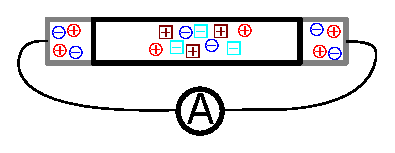
\includegraphics[width=1\textwidth]{displacement_current/first.pdf}
						\subcaption{Initial condition}\label{fig:displacement_current-initial}
					\end{subfigure}
					\bigskip

					\begin{subfigure}[t]{0.5\textwidth}
						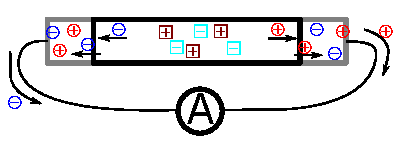
\includegraphics[width=1\textwidth]{displacement_current/second.pdf}
						\subcaption{Free charges crossing interfaces}\label{fig:displacement_current-electronic}
					\end{subfigure}
					\qquad
					\begin{subfigure}[t]{0.5\textwidth}
						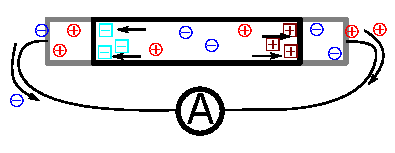
\includegraphics[width=1\textwidth]{displacement_current/third.pdf}
						\subcaption{Ions accumulating at interfaces}\label{fig:displacement_current-ionic}
					\end{subfigure}

					\mycaption[Representation of current and displacement current.]{(\textbf{a}) a mixed ionic-electronic conductor material layered between two layers of electronic conductor material.
						(\textbf{b}) the electronic charge can cross the material's interfaces.
						(\textbf{c}) ionic charge cannot be transferred to the electrodes, still a displacement current due to the ionic migration is generated and can be measured in the amperometer.}\label{fig:displacement_current}
				}
			}
		\end{figure}


		\paragraph{Displacement current -- interpretation} So the displacement current accounts for the charge movements not identifiable as current and for their effect on the surrounding circuitry.
		An example is represented in \cref{fig:displacement_current-ionic}: the amperometer can measure a current even if no charge crossed the perovskite/electrode interface, this is a displacement current caused by the creation of a dipole due to the ionic accumulation at the interfaces.
		One can imagine the resulting current as needed for maintaining the zero potential difference between the two contacts.
		It is not, as one could erroneously and instinctively think, the effect of an electric field generated in the contacts by the moving charge in the perovskite layer (with related Coulomb force and image charges) as out of the two two-dimensional planes of opposed charges no electric field is present.
		This can be understood thinking that the electric field intensity generated by a large plate of charges has a constant magnitude at distances much smaller than the plate dimensions (which is always true in our solar cells considering the thickness \SI{\approx 1}{\um} to area \SI{3x3}{\square\mm} ratio, except at electrode edges).
		The concept is represented in \cref{fig:dipole_plane}.
		In \cpageref{displacement_current_ionic} we'll use the displacement current concept for simulating the current caused in the electrodes not by a net flux of charges through a device section but by the rearrangement of charges which not necessarily leave the device, like the ionic migration in perovskite material.

		\begin{figure}
			\makebox[\textwidth][c]{
				\parbox{1.1\textwidth}{
					\centering
					\begin{subfigure}[t]{0.41\textwidth}	\centering
						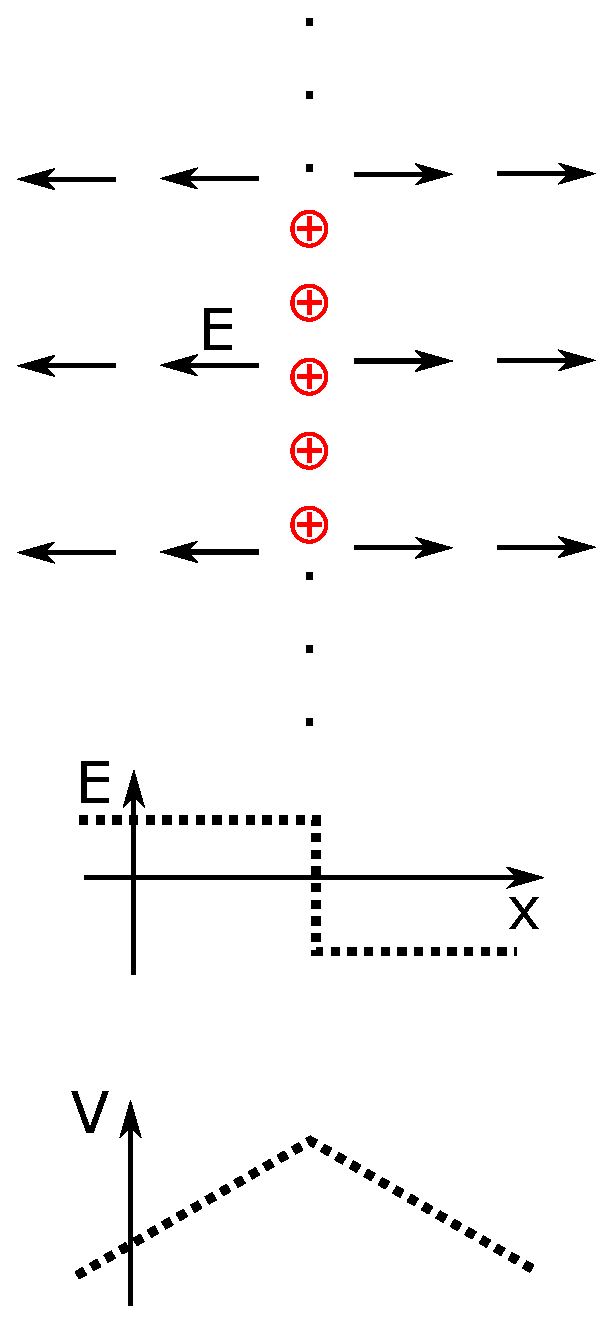
\includegraphics[height=0.3\textheight]{dipole_plane/single.pdf}
						\subcaption{Infinite plane of charges}\label{fig:dipole_plane-single}
					\end{subfigure}
					\qquad
					\begin{subfigure}[t]{0.61\textwidth}	\centering
						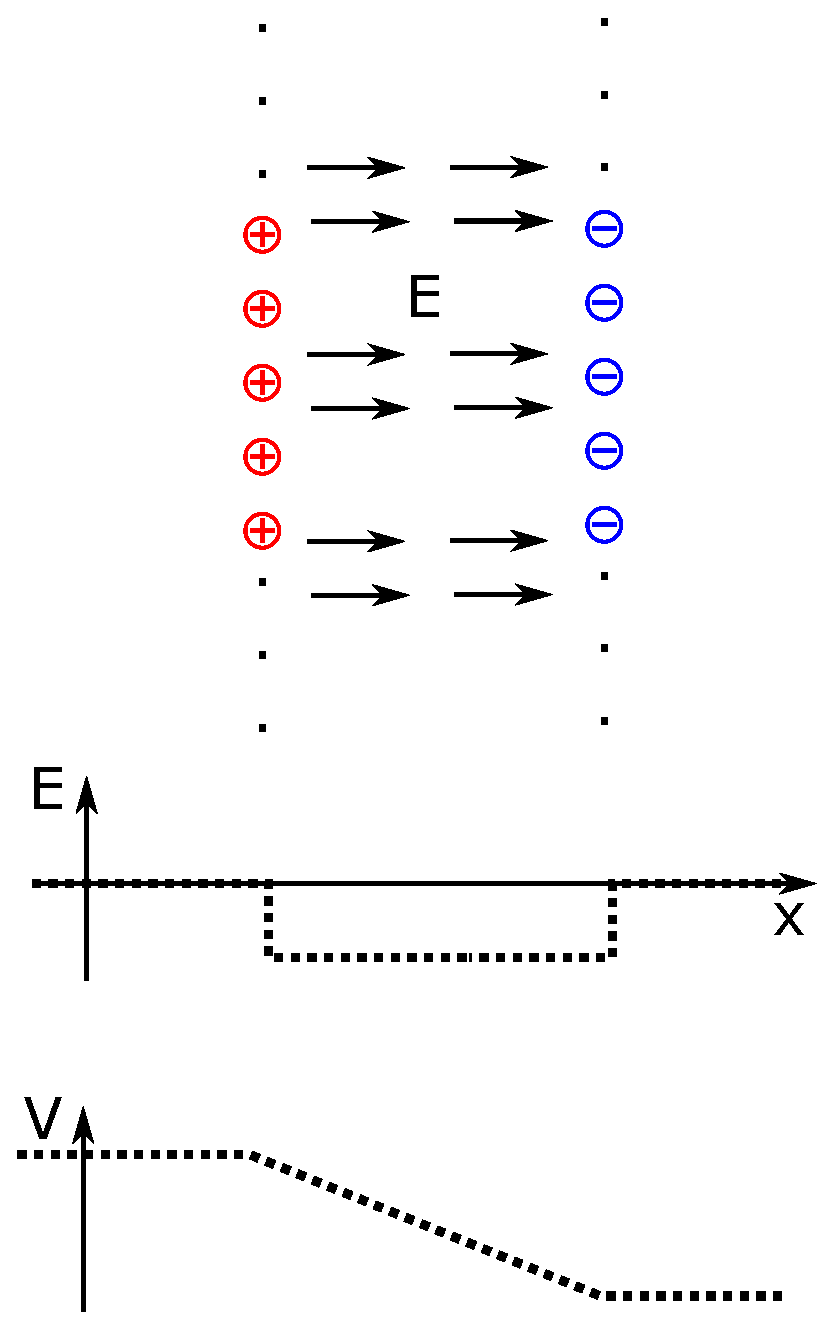
\includegraphics[height=0.3\textheight]{dipole_plane/double.pdf}
						\subcaption{Two infinite planes of opposed charges}\label{fig:dipole_plane-double}
					\end{subfigure}

					\mycaption[Electric field by two planes of opposite charges.]{(\textbf{a}) an infinite plane of charged particles is represented, the electric field is constant on the two sides, with a discontinuity in the plane.
						(\textbf{b}) adding a second plane with the same concentration of charges of the opposite kind, the electric field out of the sandwich cancels out.
						What is present outside of the sandwich is just an electrostatic potential difference.}\label{fig:dipole_plane}
				}
			}
		\end{figure}

		\paragraph{Continuity equation}
		The continuity equation has a very intuitive meaning: the concentration of a specie in a specific volume can increase due to generation $g$, can decrease due to recombination $U$ or can change due to a speed change of a charge flow passing by.
		This last contribution can be understood with the following example: a traffic light stops the cars flow and causes the increase of their concentration.
		For electron concentration $n$:
		\begin{equation}\label{eq_continuity}
			\frac{\partial n_x}{\partial t} = \frac{1}{q}\nabla_x \cdot J_n + g_{n,x} - U_{n,x}
		\end{equation}

	\subsection{Charge Recombination}

		\paragraph{Primary geminate recombination} \label{intro_geminate}
		This kind of recombination happens with the annihilation of a photo-generated exciton prior to the free charges separation.
		This is independent from the illumination intensity, so it can be considered as having a reaction order of zero.
		Lead halide perovskite have quite a high static permittivity \cite{Moia2019} and a small electron effective mass \cite{Herz2017} which means a high holes and electrons mobility \cite{Leijtens2014}, this means that, at room temperature, the exciton binding energy (described in \cpageref{intro_exciton}) is even smaller than $k_|B|T$ \cite{Miyata2015,Galkowski2016,Tvingstedt2015} and the direct generation of free charges occurs.
		So this kind of recombination is negligible in perovskite solar cells \cite{Wehrenfennig2014}.
		%Non-geminate recombination refers to the annihilation of an electron and an hole happening after their complete separation, as opposed to geminate recombination where the recombination happens just after the charges separation but before their distancing.

		\paragraph{Radiative recombination}
		This is an unavoidable form of recombination, which finds its origin in the detailed balance principle describing that, at steady state, all the absorbed thermal photons, coming from the surroundings of the cell, have to be re-emitted as black body radiation.
		From this parallelism it can be understood that this recombination is larger for materials with greater absorptivity \cite{Nelson2003} like the ones used for thin film solar cells \cite{Tvingstedt2015}.
		An indirect bandgap disfavours the radiative recombination: in these materials the recombination involves a large momentum variation, while the photon emitted due to the recombination can take just a small momentum and the rest of it should be released as an additional phonon (lattice vibrations).
		Radiative recombination involves the collision of two opposite free charges, so it can be considered as having a reaction order of 2 when electrons and holes concentrations are similar, $n \approx p$ (in intrinsic semiconductors out of the depletion layer or, in intrinsic perovskites, once ionic profile stabilized cancelling the electric field), while in case of uneven concentrations (in doped semiconductors or inside depletion layers) the limiting reagent is the minority carrier (electrons in p-type and holes in n-type materials) and the reaction order is 1.
		The expression used for modelling is:
		 \begin{equation}
		U_|rad| = k_|rad| (np-n_|i|^2)
				\end{equation}
		where $n_|i|$ is the equilibrium carrier density as obtained from Boltzmann distribution for an intrinsic semiconductor, it is just introduced in the equation in order to account for the thermal generation.
		The dependency from $np$ indicates that this recombination type depends on the quasi\hyp{}Fermi levels splitting.
		This type of recombination is present in perovskite solar cells, indeed some of the most efficient perovskite solar cells can be used as \gls{led} taking advantage of their radiative recombination \cite{Bi2016}.

		\paragraph{\gls{srh} trap mediated recombination}
		Also known as Shockley-Read-Hall recombination \cite{Shockley1952}, this recombination happens in two steps: a free charge from the respective band decays into an empty localized state with energy in between the valence and the conduction bands, a trap, after this event, a free charge of the opposite sign reaches the trapped charge location and recombine with it.
		As aforementioned, in an indirect band gap material the radiative recombination is disfavoured, but the presence of a trap state can divide in two easier steps the charge recombination process.
		%		In an indirect band gap material (where the momentum difference between the starting and final state is large) band-to-band bimolecular radiative recombination is disfavoured, but the presence of a localized trap state can catalyse the transition 
		Usually both the momentum difference and the chemical energy is released \textsl{via} phonons, so no radiative emission is involved.
		This recombination type can have reaction order of 1 or 2 depending on how many of these steps constitutes a bottleneck \cite{Calado2019}.
		In case of mid-gap traps (with energy in the middle of the bandgap), these states will be rather saturated and the process of trapping a free charge will be slow as an empty trap has to be hit, then the actual recombination is fast, so the reaction order is 1.
		In case of shallow traps, the first step could or could not be a bottleneck, this time depending on the availability of free charges to trap: in doped semiconductors this could be a limiting factor, and the reaction order would be again 1; in intrinsic semiconductors there will be plenty of free charges of both types, and the reaction order can get close to 2.
		The expression used for modelling is \cite{Shockley1952,Nelson2003}:
		\begin{equation}\label{eq:srh}
			U_{SRH} = \frac{np-n_|i|^2}{\tau_n(p+p_t)+ \tau_p(n+n_t)}
		\end{equation}
		where $\tau_n$ and $\tau_p$ are constants describing the trap capture cross section (which can be different for electrons and holes) and the traps density while $n_t$ and $p_t$ are the carrier densities that would be present with a the Fermi level equal to the traps energy.
		For a doped semiconductor with similar $\tau_n$ and $\tau_p$, the expression can be simplified, for example in a p-type material we can use \cite[108]{Nelson2003}:
		\begin{equation}
		U_{SRH} \approx \frac{n-n_0}{\tau_n}
		\end{equation}
		so, the more the material is densely doped, the smaller the minority carriers density and the less important is this kind of recombination.
		For lead halide hybrid perovskite materials, this kind of recombination is or is not important depending on the presence of mid-gap states, which in turn depends on the material composition and stoichiometry.

		\paragraph{Surface recombination}\label{intro_surface_recombination}
%		Also known as interfacial recombination, refers to the annihilation of one kind of free charge on a material with a charge of the opposite sign located on another material, happening at the materials' interface.
		Also known as interfacial recombination, refers to the annihilation of two opposite charges happening at the boundary of a material block: an interface.
		An interface can form between grains of the same material or between different materials.
		At the boundary of a crystal, the well ordered structure is interrupted creating various localised states which can act as traps for \gls{srh} recombination.
		Additionally, the impurities tend to accumulate to the crystalline grain surface, external contamination is likely to occur at the material surface, chemical reactivity can vary the composition of two materials' interface, and mid-gap states could be already present in one of the two interfacing materials.
%		The presence of mid-gap states in the doped selective contact can mediate the recombination in a fashion similar to the aforementioned Shockley-Read-Hall mechanism.
		In this thesis, I will consider the surface recombination as a case of \gls{srh} recombination.
		Considering the interface between two different materials, for example, p-doped \gls{htm} and close-to-intrinsic perovskite, the surface recombination will involve the majority carrier, holes, in the doped material and electrons in the intrinsic semiconductor.
		As the doped semiconductor has abundance of majority carriers, the limiting factor will be the concentration of "minority" carriers on the other side of the interface, which will depend on its mobility and on the electric field in the intrinsic.
		So the reaction order should be 1 for this case.
		In efficient perovskite solar cells, this is the most important recombination pathway \cite{Calado2019,Carnie2015,Stolterfoht2018a}, at least for aged devices \cite{Tress2018,Correa-Baena2017a}.

		\paragraph{Auger recombination}
		When a free charge gets in contact with another of the same kind, it is possible that one of these decays and the other absorbs the just released energy as kinetic energy.
		Additionally to the two free charges of the same kind, it also requires a free charge of the opposite kind for the decay to be possible, so it can be considered as having a reaction order of three.
		This recombination is important in materials with high free carriers densities or at high photo-generation conditions.
		These high charge densities are unlikely to happen in perovskite solar cells at normal working conditions.

	\subsection{Charge Generation}
	Thanks to microscopic reversibility, each of the mentioned recombination processes has an identical but opposed generation process \cite[81]{Nelson2003}.
	These generation processes require some energy in input, which can be thermal (phonons, lattice vibrations) for the generation associated to the non radiative processes or radiative for the reverse of the radiative recombination.
	This last case, named photogeneration, is the most interesting for photovoltaics.



		\paragraph{Light absorption}
		Photons entering a material can be absorbed depending on their energy.
		This is closely related to the material polarizability (permittivity): imagine a molecule like a metallic stick and the incoming photon as its associated electric field wave.
		The electric field would cause the electrons and the holes inside the metallic stick to accumulate at its two opposite extremities, increasing its internal energy.
		The energy gained by the stick would absorb all the energy of the incoming electric field, causing the annihilation of the photon.
		Passing to consider a molecule, the photon would be absorbed just if it matches the energy difference between an occupied and a virtual electronic states and just if the dipole vector of the starting state is not identical to the final state (and more selection rules).
		After the photon absorption, the previously occupied energy level is now missing one electron which has been promoted to the previously virtual state.
		This is represented in \cref{fig:generation-excited_hot} for a high energy photon generating a hot excitation \ch{M^{*h}} (which later can result in a hot exciton and a hot carrier, not treated in this thesis) or in \cref{fig:generation-excited} for a photon with just enough energy to generate an excitation \ch{M^{*}}.
		Photons with energy smaller than the optical band gap can also be absorbed by different processes like valence band to empty mid gap localised state, occupied mid gap localised state (trapped charge) to conduction band but they will not be considered in this thesis.
		
		\begin{figure}
			\makebox[\textwidth][c]{
				\parbox{1.1\textwidth}{
					\centering
					\begin{subfigure}[t]{0.25\textwidth}
						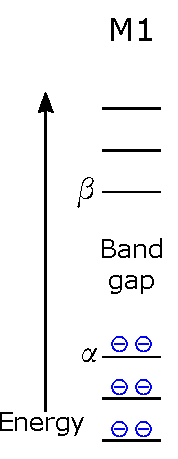
\includegraphics[scale=0.8]{generation/initial.pdf}
						\subcaption{\\Initial state}\label{fig:generation-initial}
					\end{subfigure}
					\qquad
					\begin{subfigure}[t]{0.2\textwidth}
						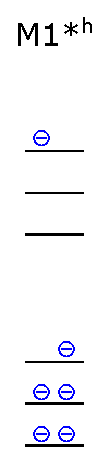
\includegraphics[scale=0.8]{generation/excited_hot.pdf}
						\subcaption{\\Hot excitation}\label{fig:generation-excited_hot}
					\end{subfigure}
					\qquad
					\begin{subfigure}[t]{0.2\textwidth}
						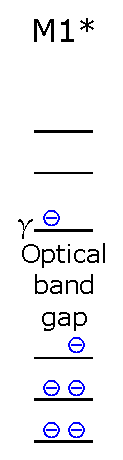
\includegraphics[scale=0.8]{generation/excited.pdf}
						\subcaption{\\Excitation}\label{fig:generation-excited}
					\end{subfigure}
					\qquad
					\begin{subfigure}[t]{0.22\textwidth}
						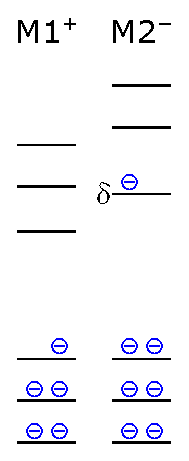
\includegraphics[scale=0.8]{generation/exciton.pdf}
						\subcaption{\\Exciton}\label{fig:generation-exciton}
					\end{subfigure}
					\mycaption[Representation of absorption and generation of an exciton.]{
						In (\textbf{a}) the fundamental molecular electronic configuration is represented, for the meaning of the levels refer to \cref{fig:homo_lumo}.
						In (\textbf{b}) a photon with high energy excited an electron from the \gls{homo} to the \gls{lumo}$+2$, equivalently also other levels can be involved \textsl{e.g.} \gls{homo}$-1$.
						In (\textbf{c}) a photon with just enough energy has promoted an electron.
						Please note that the final state of the electron (a \gls{somo}) has a lower energy than the \gls{lumo}, as explained in the text.
						In (\textbf{d}) the excited electron in the \gls{somo} has been transferred to the \gls{lumo} of an adjacent molecule. 
					}\label{fig:generation}
				}
 			}
		\end{figure}
	
		\paragraph{Exciton and exciton binding energy}\label{intro_exciton}
		The starting state of the electron involved in the radiative excitation is the \gls{homo} of the molecule \ch{M}, marked in \cref{fig:generation-initial} with $\alpha$.
		When an electron is removed from the \gls{homo}, the energy of the \gls{lumo} decreases, as it now refers to a different electronic configuration, where the underlying orbitals are not fully balancing the nuclei positive charges any more.
		So the arrival state of the excited electron, marked with $\gamma$ in \cref{fig:generation-excited}, is at a lower energy than the initial state \gls{lumo} ($\beta$) and the optical band gap (which can be measured from absorbance spectrum \textsl{via} a Tauc plot) is smaller than the band gap (difference between the electron affinity and the ionization potential represented in \cref{fig:homo_lumo}).
%		The \gls{lumo}, marked as $\beta$, gets occupied by the promoted electron and its energy decrease, to the new level with $\gamma$ in .
%		As can be seen comparing the $\beta$ and the $\gamma$ levels, 
		Next to the excitation, an electron can either go back (recombine) or start getting apart from the original location, as represented in \cref{fig:generation-exciton} where it has been transferred to an adjacent molecule.
		As a final step for generating a free carrier, the Coulomb force caused by the electron on \ch{M-} and the "hole" on \ch{M+}.
		Both the aforementioned energy difference between $\gamma$ (upper \gls{somo} of the excited molecule) and $\delta$ (\gls{lumo}), and the energy needed for taking the charges apart breaking the electrostatic attraction of the exciton contribute to the exciton binding energy.
		For most of the crystalline materials with delocalized orbitals, electron binding energy is smaller than the ambient thermal energy $k_|B|T$ so a direct generation of free charges moving independently is observed.
%		Also localised states (charges in mid gap traps) can be involved in optical excitation, in that case
%		\paragraph{Light absorption in presence of electric field}\label{intro_electroabsorbance}

	\subsection{PhotoVoltaic Effect}
	The charge generation causes an increase of the concentration of both electrons in the conduction band and of holes in the valence band.
	This can be represented with the position of the quasi\hyp{}Fermi levels as their approach to the respective band edge ($E_|fn|$ towards conduction band and $E_|fp|$ towards valence band).
	
	
	\begin{figure}
		\centering
		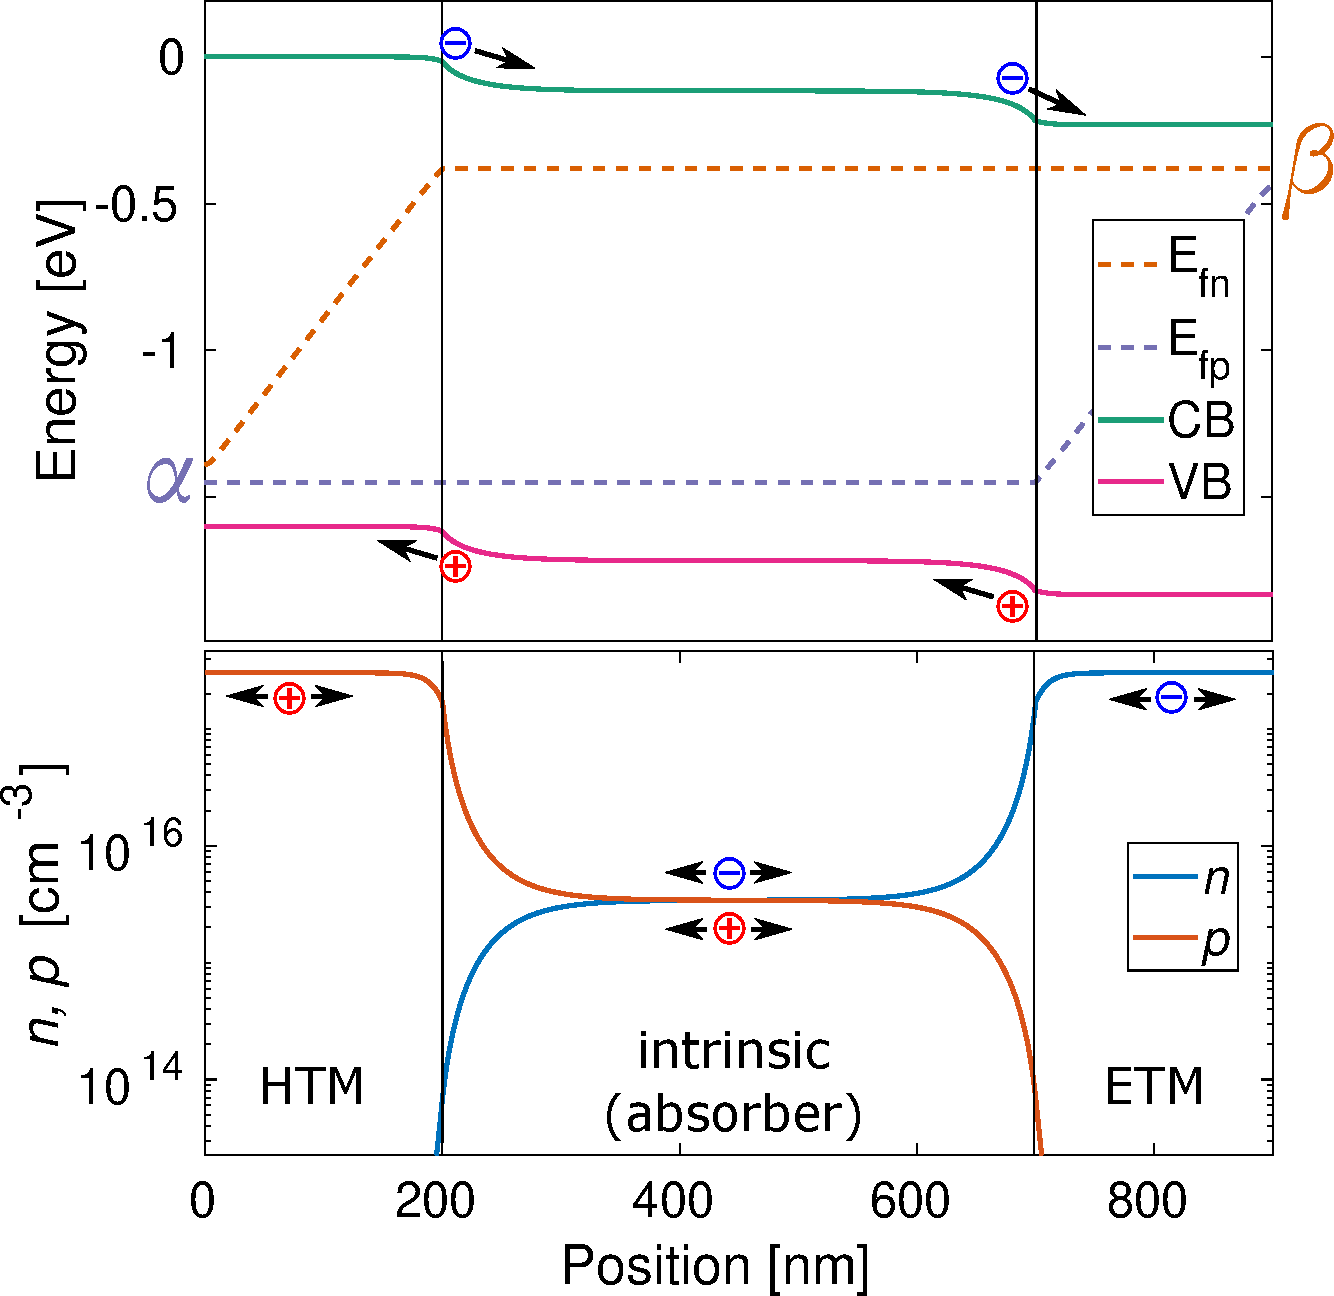
\includegraphics[width=0.7\textwidth]{collection/OC_noions_loweppAbsorber-annotated.pdf}
		\mycaption[Simulation of a p-i-n homojunction device illuminated at open circuit.]{
			From left to right: p-type material, intrinsic semiconductor where generation occurs, n-type material.
			Low permittivity in the central layer was employed in order to represent also an electric field free zone.
			In top figure, the band diagram is represented.
			Single arrows indicate drift due to the field.
			The observable gradients of the quasi-Fermi levels just represent the minority carriers recombination current.
			The values of $E_|fp|$ in the location marked with $\alpha$ and of $E_|fn|$ in $\beta$ are the relevant ones for the open circuit voltage.
			In bottom figure: the charges' concentrations.
			Double arrows represent charge diffusion.
		}\label{fig:collection}
	\end{figure}
	
		\paragraph{Charges reaching the interfaces \textsl{via} diffusion}
		In the absorber layer (the material where light gets absorbed), the charges concentration increases thanks to the generation, this causes a gradient of concentration that drives a diffusion current (see \cpageref{intro_diffusion}) towards the non\hyp{}absorbing layers.
		At the interface with the contacts, the carriers' concentration is often smaller than in the bulk and this keeps up the diffusion current.
		This happens either due to recombination processes at the interfaces (e.g. when an electron reaches the holes rich p-type \gls{htm}) or to the charges collection through the interfaces as described in the next paragraph.
		As we will see, in perovskite solar cells the electric field in the bulk is mostly screened, and the transport \textsl{via} diffusion is very important.
		In the exampled reported in \cref{fig:collection}, the gradients in the charges' concentrations cause diffusion currents.
		
		\paragraph{Charge collection due to drift}
		In regions where an electric field is present, \textsl{e.g.} close to the interfaces in a perovskite solar cells, the free charges are pulled by the Lorentz force as seen in \cpageref{intro_drift}.
		In the exampled reported in \cref{fig:collection}, the curvature of the bands indicates the presence of electric field driving the charges' drift.

		\paragraph{Current}
		As seen above, the photogenerated electrons gets collected in the \gls{etm} and the holes in the \gls{htm} contacts.
		If an external electrical connects the two electrodes of our solar cell, optionally including a load, the accumulated carriers will discharge through this circuit and we will be able to measure a current.
		
		\paragraph{Voltage}
		The quasi-Fermi splitting induced by the photogeneration of charges gets reflected in a splitting of these levels also in the contacts.
		In the doped contacts, the concentration of the minority carrier should become negligible due to the recombination with the abundant majority carrier.
		Further, as in the metallic contacts there is no conduction nor valence band (and very fast recombination), the quasi\hyp{}Fermi level related to the majority carrier ($E_|fp|$ in the \gls{htm} or $E_|fn|$ in the \gls{etm}) is the one determining the Fermi level in the metal.
		So the difference between the $E_|fp|$ at the \gls{htm}/electrode interface ($\alpha$ in \cref{fig:collection}) and the $E_|fn|$ at the \gls{etm}/electrode interface ($\beta$ in \cref{fig:collection}) gets reflected into the electrodes Fermi level, which ultimately can be measured as a voltage.
			 
%		For this reason the relevant energy level at the left end of \gls{htm} is the valence band quasi\hyp{}Fermi level $E_|fp|$ 

\section{Perovskite Solar Cells}
	\epigraph{\textit{\enquote{That's yogurt science!}}}

\begin{SCfigure}
	\centering
	\includegraphics[width=0.5\textwidth]{nrel_chart/pv-efficiencies-2019-01-03.pdf}
	\mycaption[NREL chart of "Best Research-Cell Efficiencies"]{Just the perovskite solar cells (not stabilized) results have been reported.}\label{fig:nrel_chart}
\end{SCfigure}

	Lead perovskites are known since long time, both inorganic \cite{Moller1958} and hybrid inorganic\hyp{}organic \cite{Weber1978}.
	Just recently, in 2009, it has started to be used as absorber for solar cells (started by the research groups Miyasaka \cite{Kojima2009}, Park \cite{Im2011a,Kim2012b}, and Snaith \cite{Lee2012}).
	Perovskite solar cells evolved from the \gls{dssc} tradition, where an absorber dye is in contact with a titania \gls{etm} and an organic \gls{htm}.
	Here the absorber dye is substituted by a hybrid organic-inorganic lead halide perovskite semiconductor and both the \gls{etm} and the \gls{htm} can be composed of various, either organic or inorganic, materials.
	Thanks to the enormous research effort, these kind of devices reached a record stabilized efficiency of 20.9~\% \cite{Green2019} with reports of even higher non-stabilized efficiencies (23.7~\% \cite{Green2019,Jiang2017}); all this in relatively short time as represented in \cref{fig:nrel_chart}.

%	\paragraph{Composition}
%	Cesium introduction \cite{Bi2016,Saliba2016}


\begin{figure}
	\makebox[\textwidth][c]{
		\parbox{1.1\textwidth}{
			\centering
			\begin{subfigure}[t]{0.45\textwidth}
				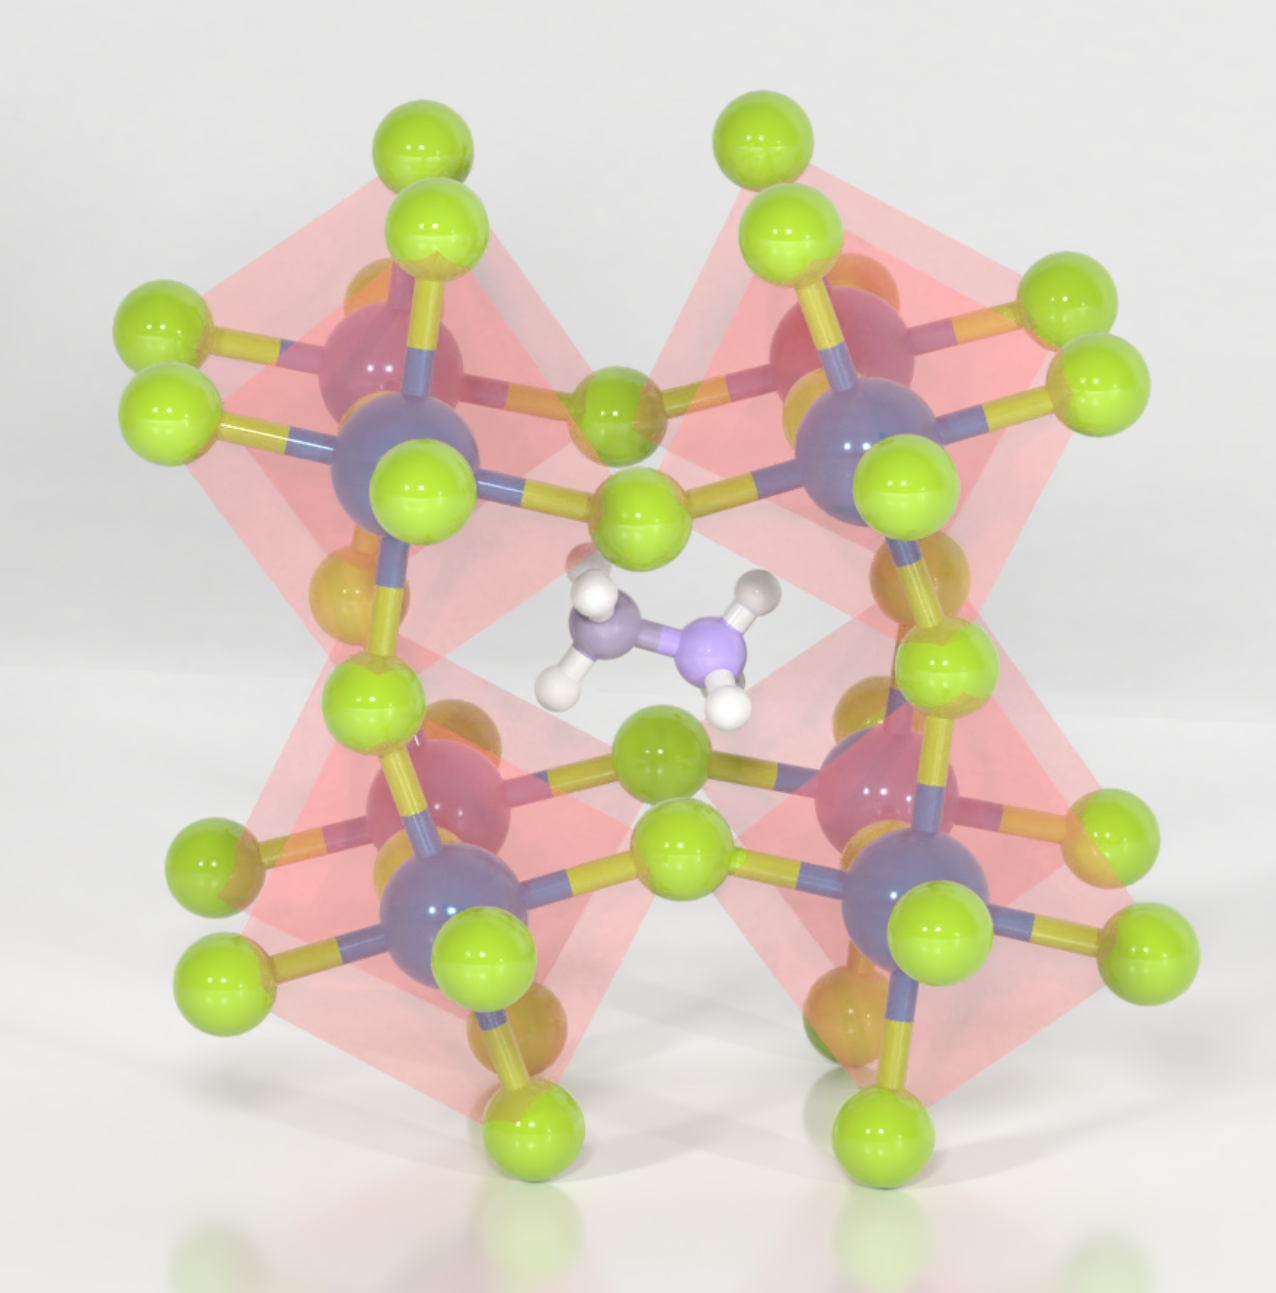
\includegraphics[width=1\textwidth]{crystal_perovskite_edvin_fako/ilario2-crop.jpg}
				\subcaption{}\label{fig:crystal-single}
			\end{subfigure}
			\qquad
			\begin{subfigure}[t]{0.57\textwidth}
				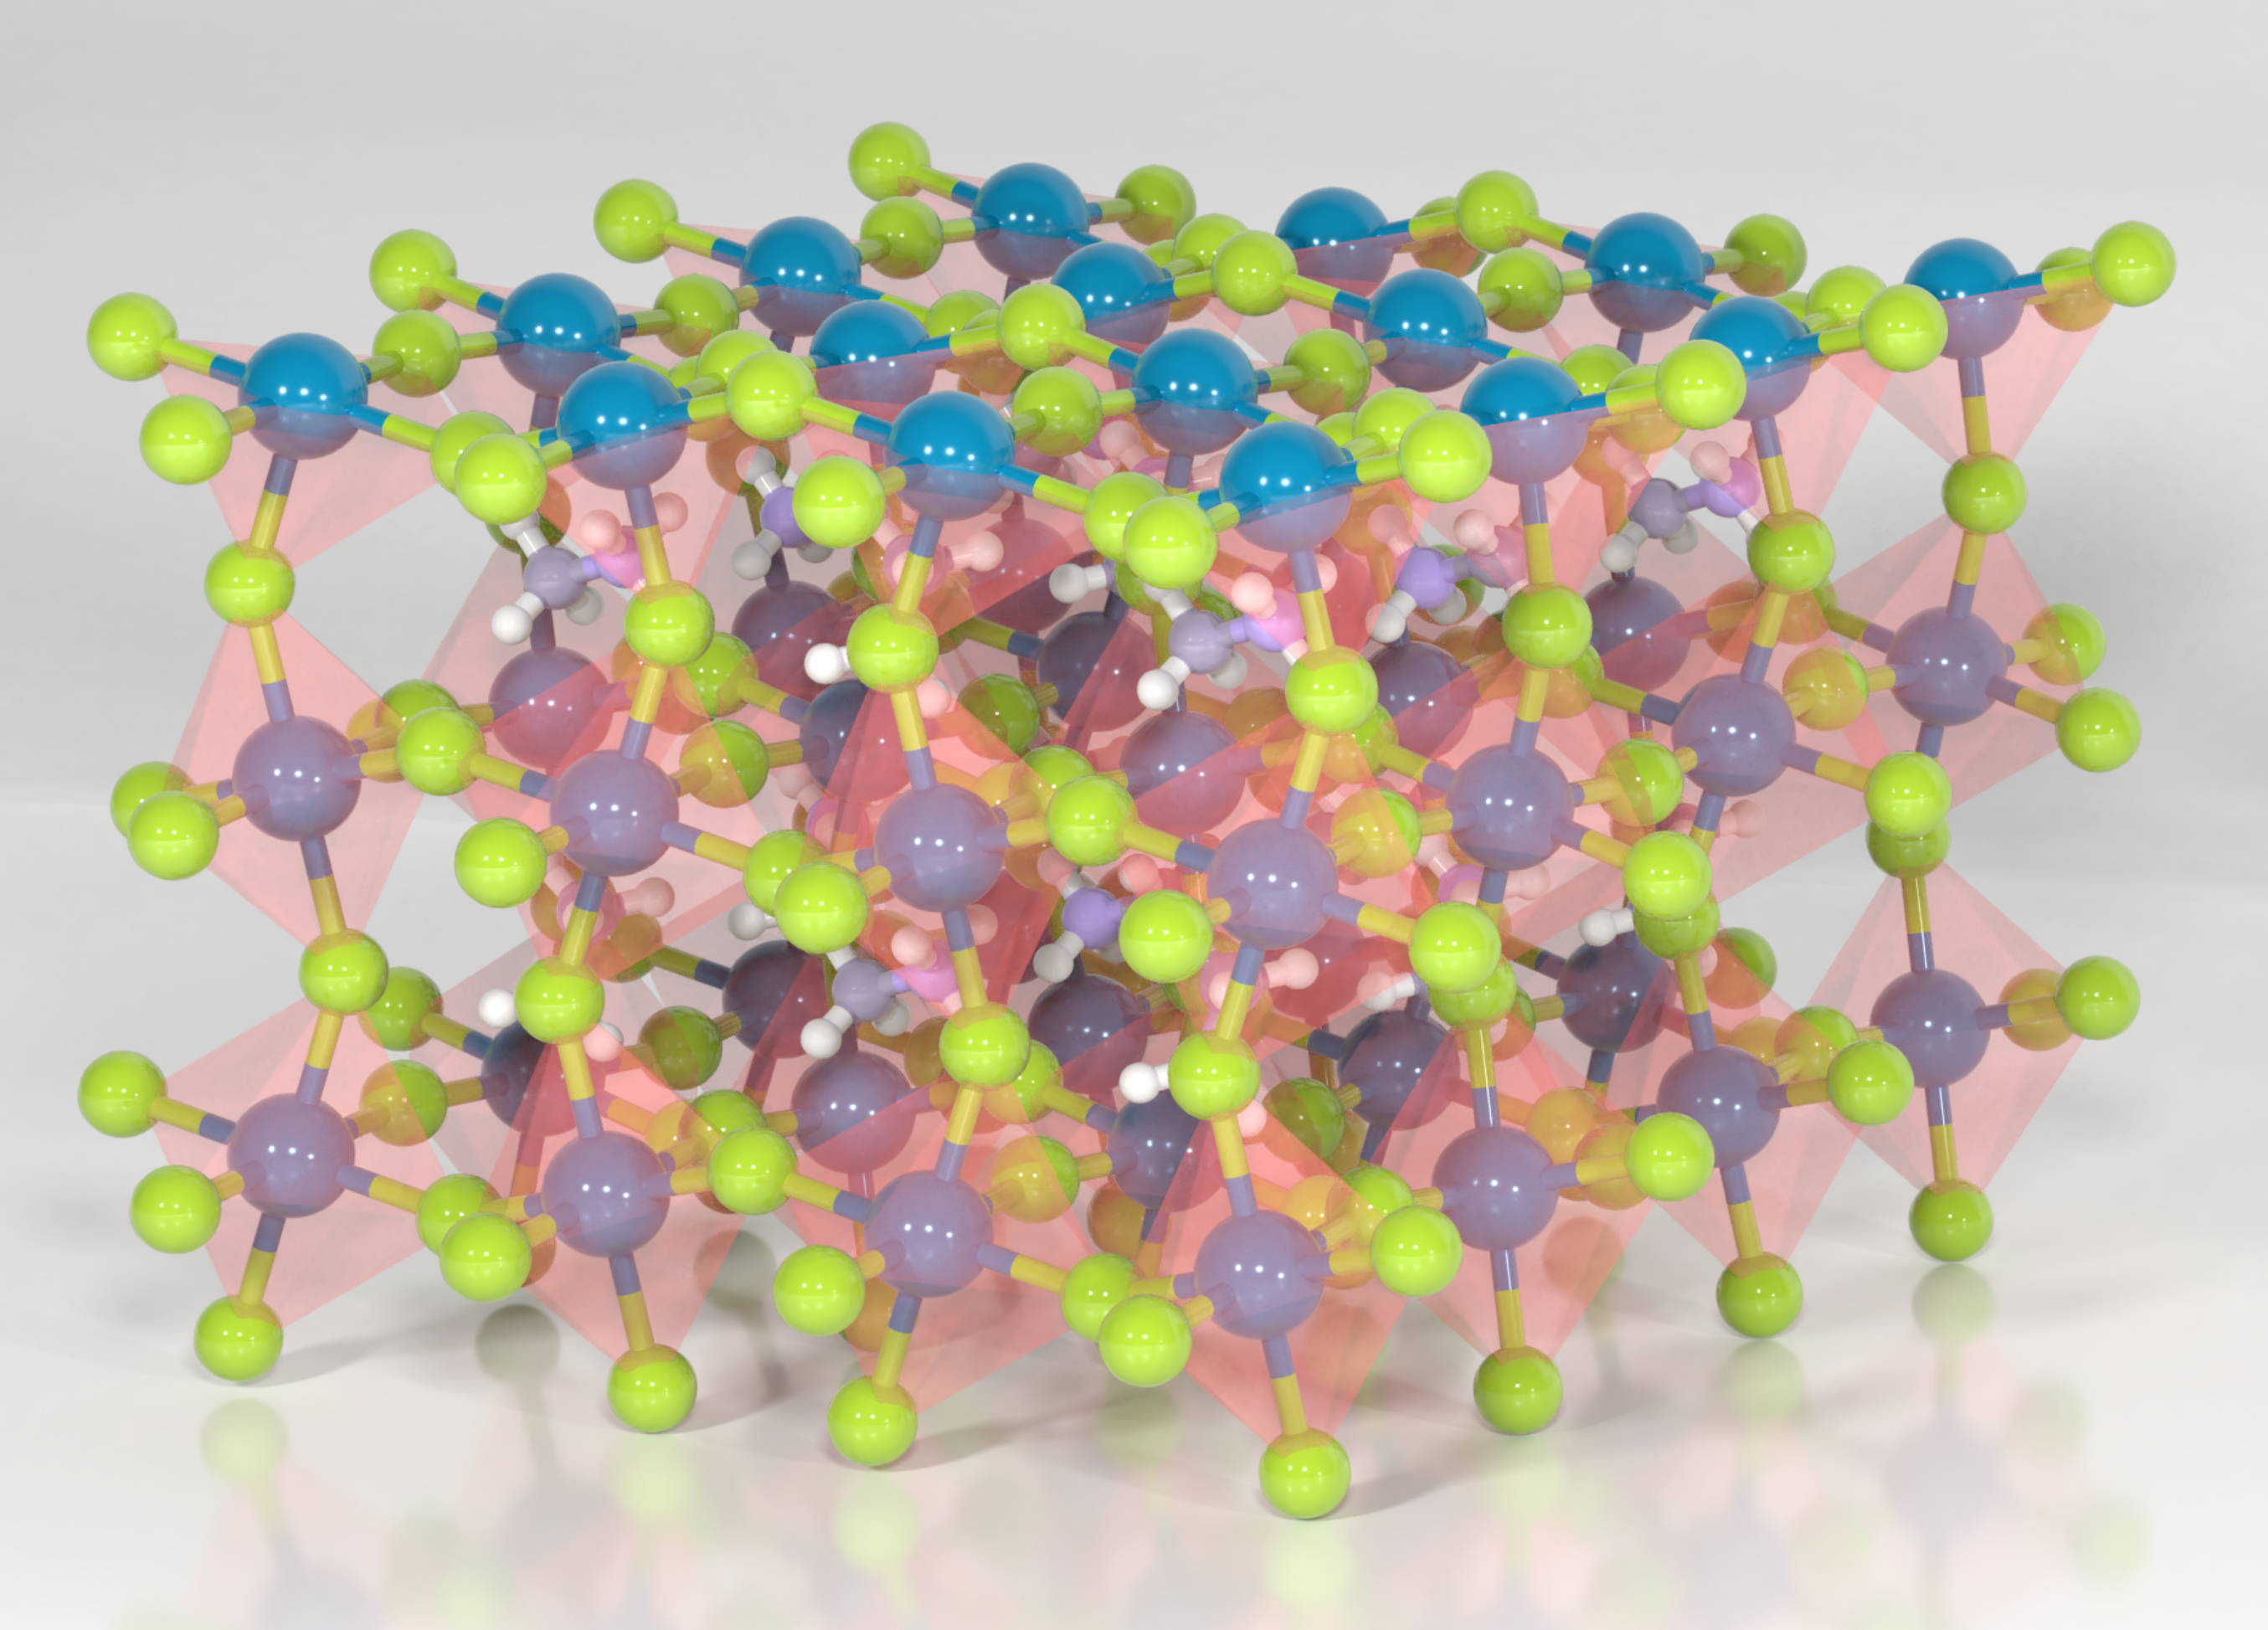
\includegraphics[width=1\textwidth]{crystal_perovskite_edvin_fako/ilario1-crop.jpg}
				\subcaption{}\label{fig:crystal-bulk}
			\end{subfigure}
			\mycaption[Crystal structure of \glsentrytext{mapi} perovskite.]{In (\textbf{a}) the methylammonium cation is between \ch{PbI6} octahedra.
			In (\textbf{b}) the bulk structure is represented.
		These graphics, created with Vasp and Blender software, are courtesy of Edvin Fako \texttt{<efako@iciq.es>}.
	}\label{fig:crystal}
		}
	}
\end{figure}


	\paragraph{Perovskite Absorber Synthesis}
	The preparation of this hybrid semiconductor \textsl{via} spin coating and annealing at low temperature is extremely easy and convenient for small-scale research purposes.
	%	From my point of view, 
	Nevertheless, this fabrication process is affected by a low reproducibility, likely due to the sensibility of the drying and crystallization step \cite{Pockett2015}.
	This factor clearly slows down the research in perovskite solar cells.
	In literature various reports of completely different results obtained from supposedly identical synthesis can be found \cite{Pockett2015,Gottesman2014}.
	This issue is being addressed recently with the publication of more reliable and complete fabrication procedures \cite{Saliba2018}.

	\paragraph{Recombination mechanisms}\label{intro_prv_recombination}
	The non-radiative recombination inside the perovskite material is surprisingly low for a low temperature processed material.
	This is demonstrated by the large diffusion length in isolated crystals \cite{Wehrenfennig2014,Wehrenfennig2014a,Stranks2013,Xing2013,Shi2015a,Eperon2014}: for the \gls{csfamapbibr} it is reported being \SI{\approx140}{\nm} for the electrons and \SI{\approx1.9}{\um} for holes \cite{Liu2017}.
	This is confirmed by the fact that once a thin layer (\SI{\approx500}{\nm}) of the material is layered between an \gls{etm} and an \gls{htm} the photoluminescence lifetime is dramatically reduced \cite{Jimenez-Lopez2017,Eperon2014} indicating that the free charges can diffuse at least over the layer thickness.
	Even if not always the case \cite{Valadez-Villalobos2019,Tress2018,Peng2016}, it is often reported that at open circuit conditions, the predominant recombination pathway in perovskite solar cells is identifiable as the surface recombination at the perovskite/selective contacts interfaces \cite{Calado2019,Stolterfoht2018a,Stolterfoht2018,Gelmetti2019,Shao2016,Correa-Baena2017,Hou2016}.
%		This recombination is more important in a perovskite solar cell rather than in \gls{osc} as the built-in field is shielded by the ionic accumulation and the minority carriers concentration at the perovskite\-/contacts interfaces is higher.
This recombination is important in perovskite solar cells also due to the high minority carriers concentration close to the contacts, which is a result of the screening of the electric field in the bulk of the perovskite material.
%This recombination is more important in a perovskite solar cell rather than in \gls{osc} as the built-in field is shielded by the ionic accumulation and the minority carriers concentration at the perovskite\-/contacts interfaces is higher.
	%	Considering the perovskite material, traps are more likely to form on the surface of crystal domains, where the bulk symmetry is broken and carrier-phonon coupling, which can ease indirect transitions is more likely due to the easier deformation of the broken structure . 

	\paragraph{Open circuit voltage}
	The open circuit voltage of a perovskite solar cell depends on many contributions and has a hard upper limit dictated by the perovskite band gap and the radiative recombination \cite{Tress2017,Tress2015a}.
	This recombination is unavoidable as it originates by the detailed balance for a strongly absorbing material \cite[24]{Nelson2003}
	As we will see in \cref{ch:characterization}, the aforementioned surface recombination rate is one of the other contributions.
	Such non\hyp{}radiative recombination has been predicted to have influence on the \gls{voc} of perovskite solar cells when the relative life time is smaller than \SI{10}{\us} \cite{Tress2017}.
	A contact material having mid-gap states will favour the surface recombination, but also its additives (\textsl{e.g.} dopants, dispersants\dots) can introduce such trap states \cite{Correa-Baena2017}.
	Additionally, a different material employed as \gls{etm} and \gls{htm} will result in a different built-in voltage (difference in contacts' Fermi levels energies), which constitutes a limit for the the open circuit voltage \cite{Gelmetti2019,Wu2016} in case the surface recombination is the main loss mechanism \cite{Tress2017}.
	The presence of ionic accumulation in perovskite solar cells have been reported to reduce the influence of the \gls{voc} from the built-in voltage \cite{Belisle2016}.
	Even a different molecular ordering in the selective contacts can influence the \gls{voc} through the variation of the \gls{dos} width, and by consequence the energetics of the band edges \cite{Shao2016}.
	Rather than a hard limit, the built-in voltage represents the applied voltage that saturates the depletion layers in the contacts, which implies a large charge density at the materials interface and an important surface recombination \cite{Gelmetti2019,Kirchartz2019}.
	Indeed, it has been predicted that suppressing the surface recombination can allow a device to give a voltage higher than the built-in voltage \cite{Kirchartz2019}.
	A large absorber band gap will have the excited charges thermally relaxing to a more energetic band, allowing the solar cell to achieve a higher \gls{voc}.
	The perovskite band gap can be easily tuned changing its stoichiometry, for example partially replacing iodine with bromine \cite{McMeekin2016,Noh2013a,Wheeler2017} or using different organic cations \cite{Eperon2014}.
	For perovskite solar cells, the record reported \textit{bandgap\hyp{}voltage offset} are already much smaller than the voltage losses reported for \gls{osc} \cite{Tvingstedt2015}.
	Also the morphology and composition of perovskite material can have an impact on the \gls{voc}: non-passivated perovskite surface states which can act as traps \cite{Zheng2017} thanks to the easier deformation of the broken crystal cell, favouring the electron-phonon coupling needed for indirect transitions \cite{Wu2015}; inhomogeneous perovskite layer can lead to pinholes and direct recombination between the two contacts \cite{Lee2015,Montcada2017,Qiu2016,Marchioro2014}; accessible grain boundaries due to non-compact perovskite layer causes the presence of more recombination centres \cite{Shao2016a}; the presence of secondary phases with in-gap energies can be reduced modifying the perovskite composition \cite{Bi2016}.
	If we consider the possibility of stabilising the hot carriers (free charges generated by a photon with energy larger than the band gap, can be stabilised hindering the generation of phonons needed for their thermalisation) and of collecting them to the contacts before their thermal relaxation to the band edge, also a \gls{voc} larger than the absorber band gap could be achieved and could, at least theoretically, break the Shockley\hyp{}Queisser efficiency limit \cite{WikipediaSQlimit}.
	
%	\paragraph{Charge extraction and charge blocking}
%	Selective contacts are in charge of selectively extract one kind of charge, blocking the other.
%	Clearly, the relative position of the perovskite and selective contact energy level is key both for extraction \cite{CorreaBaena2015}
%	% and for blockage CITE SOMETHING.

\paragraph{Ionic defects}
	A Schottky defect is the lack of a ion and its counter ion from an otherwise perfect crystal structure.
	This is commonly observed in ionic solids with weak lattice energy.
	Taking as an example the \gls{mapi} lead halide perovskite, the formation of the Schottky defect \ch[kroeger-vink=true]{V'_{MA} + V^._{I}} (a methylammonium cation and a iodine anion leaving the crystal) is expected to be rather easy as these ions leaves behind vacancies with just charge $\pm 1$ and the product, \ch{CH3NH3I} can further decompose in volatile compounds like methylamine and hydrogen iodide.
	Indeed, the enthalpy of formation of this defect has been calculated to be only \SI{0.08}{\eV}, which at room temperature means that \SI{\approx 4}{\%} of the \ch{MA+} and \ch{I-} sites in \gls{mapi} are vacant \cite{Walsh2015,Yin2014}.
	This specific defect can be avoided with small variations of the stoichiometry but other kind of defects will become more likely (\textsl{e.g.} \ch[kroeger-vink=true]{V''_{Pb} + 2V^._{I}}), and the minimum defects concentration achievable with \gls{mapi} perovskite has been reported to be around \SI{\approx 8e17}{\per\cubic\cm} (\SI{\approx 0.02}{\%}) \cite{Walsh2015}.
	A iodine vacancy can also be originated by a Frenkel defect where a iodine migrates from its site to an interstitial one \ch[kroeger-vink=true]{V^._{I} + I'_{i}} and some studies support this as the origin of defects in perovskite materials \cite{Birkhold2018,Birkhold2018a,Minns2017,Mosconi2016}.
	Frenkel defects are expected to constitute shallow or deep traps in the perovskite band gap while Schottky defects should not present energies inside the band gap \cite{Kim2014h,Yin2014,Buin2014,Du2015}.
%	For a halide perovskite, when compared with an oxide perovskite where \ch{X} is oxygen, the formation of ionic defects is easier thanks to the lower charge of the ionic species which means a lower lattice energy.

	\paragraph{Ionic migration}\label{intro_ionic_migration}
	Ionic conductivity in halide perovskite materials has been pointed out more than 35 years ago \cite{Mizusaki1983,Yamada1995,Yamada1998}.
	In \gls{mapi}, the presence of mobile ionic species has been directly observed from the slowly evolving work function or a lateral device using \gls{kpfm} \cite{Birkhold2018,Birkhold2018a}.
	In a generic \ch{ABX3} perovskite, it has been shown that both the \ch{A} cation and the \ch{X} anion can migrate through the crystal \cite{SaifulIslam2000}.
	For \gls{mapi} perovskite, the majoritarian mobile species has been identified as iodine vacancy \ch[kroeger-vink=true]{V^._{I}} \cite{Yang2015e,Senocrate2017} and this is supported by a small simulated migration activation energy \cite{Eames2015,Meloni2016,Haruyama2015,Azpiroz2015,Mosconi2016a}.
	Instead, a significant contribution from methylammonium ions migration has been excluded \cite{Senocrate2018,Senocrate2017,Meloni2016}.
	In complete perovskite solar cells, the ionic migration is one of the factors causing hysteretic low frequency current\hyp{}voltage behaviour \cite{Unger2014,Xiao2015,Meloni2016,Tress2015}.
	Still, the presence of ionic motion has been demonstrated even in non\hyp{}hysteretic devices \cite{Calado2016,Jacobs2018,Bryant2015}.

	
%	The fact that in the  materials the charge of the ionic species is low, $+1$, $+2$, or $-1$, allows the crystal to form defects easily
%	The ionic defect concentration in these materials can be very high due to the weak lattice energy 
	%	The presence of and mobile ionic species have been demonstrated in various kind of hybrid lead halide perovskite materials.

	\paragraph{Field free absorber}
	The high density of ionic defects causes the equilibrium free charge concentration to be low \cite{Walsh2015} and the electric field inside the absorber to be completely shielded within few nanometres from the interfaces \cite{Tress2015}.

%	characterization complexity reduction due to more homogeneous carriers profile \cite{Kirchartz2012}

	\paragraph{Diffusion as the main transport mechanism}
	As we saw, most of the perovskite absorber layer in a perovskite solar cell will be electric field free.
	In this region, no drift will help with the charge separation and the photogenerated free charges will have to approach the contacts \textsl{via} diffusion.
	This is possible in perovskite thanks to its excellent electron and holes mobility \cite{Leijtens2014,Herz2017} making possible diffusion lengths in the micrometre scale \cite{Wehrenfennig2014,Wehrenfennig2014a,Stranks2013,Xing2013,Shi2015a,Eperon2014,Liu2017}.
	
%	(due to the built-in voltage being the workfunction difference of the selective contacts)
%	(drift is not the main transport mechanism in stabilized perovskite solar cells due to the electric screening effect of the mobile ionic species)
	\paragraph{Hysteresis}
	Hysteretic behaviour in current-voltage sweeps, while not often observed in other kind of solar cells, it is frequent in perovskite solar cells.
	Still, many reports of hysteresis-free perovskite solar cells can be found, especially for top cathode or for high performances bottom cathode devices.
	As we saw above, the presence of mobile ionic species is widely accepted for most of the hybrid lead perovskite materials and this has been indicated as one of the causes of the hysteresis \cite{Unger2014,Xiao2015}.
	Considering that the recombination and collection of free charges is affected by the ions-modulated electric field \cite{Pockett2017}, this is enough to explain the presence of hysteresis \cite{Tress2015,Calado2016} \textsl{via} the modulation of interfacial energy barriers \cite{Moia2019}.
	Additionally, adsorption or chemical reaction of perovskite ionic defects with the selective contact surface (\textsl{e.g.}\ with titanium oxide \cite{Yu2016,Beilsten-Edmands2015,Carrillo2016}) could be important and can explain why \cite{Moia2019}, bottom cathode cells with inorganic contacts usually present hysteresis while top cathode with all-organic contacts usually does not.

%	\paragraph{Intrinsic or doped semiconductor}


	\paragraph{Characterization}
	The characterization techniques for perovskite solar cells and the relative interpretation evolved from the techniques and theory built around \gls{osc} and \gls{dssc} \cite{Barnes2013}.
	This pre-existing framework has been widely used in literature for perovskite solar cells by various research groups \cite{ORegan2015b,Shao2016,Gelmetti2019,Kiermasch2018,Carnie2015}.
	Unfortunately, perovskite solar cells are different enough from \gls{osc} and \gls{dssc} to doom the utility of most of these observations.
	Moreover, while an acceptable agreement between different characterization techniques was often observed in \gls{osc} \cite{Clarke2015,Maurano2011,Foertig2012} and \gls{dssc} \cite{Barnes2013}, in perovskite solar cells we often observe hard-to-explain discrepancies \cite{Kiermasch2018}.
	In the past few years, the theoretical framework has been expanded and should finally enable the perovskite community to re-interpret and re-design the solar cells characterization techniques.
	In \cref{ch:characterization} the reader can find some of the accepted concepts and some novel proposals about the interpretation of the classical characterization techniques when used on perovskite solar cells.

	\paragraph{Stability}
	The stability of the perovskite solar cells is the number one blocker to commercialization \cite{Reyna2018}.
	Its keystone has still to be identified.
	The inclusion of self\hyp{}assembly mono layers at the materials' interfaces helps the device stability passivating surface states \cite{Lira-Cantu2017,Mingorance2018}.
	Usage of organic contact layers is also a source of instability, for example due to the slow crystallisation of \gls{spiro} \cite{Malinauskas2015} (due to its low glass transition temperature of \SI{126}{\celsius} \cite{Malinauskas2016}) and metallic oxides might be used instead \cite{Mingorance2018}.
	Also fine tuning the stoichiometry and using a mix of cations (\textsl{e.g.} adding cesium salts) can lead to a more ordered crystalline phase and reduce ionic defects concentration and mobility, both these contributions helps the stability of the devices \cite{Reyna2018}.
	An interesting investigation is being carried on by Dr.\ D.\ R.\ Ceratti and Prof.\ D.\ Cahen (unpublished) regarding the release of a proton by methylammonium cation when in contact with non-acidic materials, and thus methylamine can leave the perovskite crystal structure.
	This could explain the reports about the beneficial addition of acids in perovskite precursors solution, mainly by Snaith group \cite{Noel2017,Zhang2015a,Nayak2016}.
	Additionally, various other reactions can happen inside the material or at its interfaces, for example the formation of metallic lead \cite{Birkhold2018a,Sadoughi2015}, of molecular iodine \cite{Minns2017}, of lead iodide \cite{Buin2015,Walsh2015}, of methylammonium iodide \cite{Walsh2015}.
Some of these degradation pathways are further favoured by contact with moisture \cite{Jong2018,Schlipf2019,Hu2017,Han2015a} (which if not too much, can be reversed \cite{Leguy2015}), with oxygen in combination with light \cite{Senocrate2018a,Aristidou2017} (as described in \cpageref{methods_degradation}), with UV light \cite{Lee2016}, with temperature \cite{Philippe2015,Conings2015}, with \gls{spiro} \cite{Carrillo2016}, with \gls{pcbm60} \cite{DeBastiani2016}, with the metallic electrodes due to chemical reactivity \cite{Kato2015,Guerrero2016a,Back2016,Zhao2016,DeBastiani2016} or intermixing \cite{Domanski2016}.

%	https://www.ossila.com/pages/perovskite-solar-cell-degradation-causes

%\section{Background and Related Work}\label{sec:background}
%
%	\subsection{Perovskite Solar Cells}
%
%	\subsection{Hole Transporting Materials}
%
%	\subsection{PhotoPhysical Studies and Techniques}
%
%	\subsection{Modelling and Relevant Physics}

\section{Motivation and Aims}\label{sec:aims}
\epigraph{\textit{\enquote{To begin with, we want everything.}}}{autistici / inventati}


The objectives of this thesis are:\nolinebreak
\begin{itemize}
	\item synthesize different kinds of lead perovskite absorbers (\textsl{e.g.} \gls{mapicl}, \gls{mapi}, \gls{famapbibr}, \gls{csfamapbibr});
	\item fabricate solar cells with different structures (\textsl{e.g.} top and bottom cathode);
	\item test different materials for selective contacts, either known (\textsl{e.g.} flat or mesoporous titania, \gls{pcbm70} or plain fullerene) or novel materials obtained \textsl{via} collaborations (\textsl{e.g.} \gls{tae1}, \gls{tae3}, \gls{tae4});
	\item optimisation of the devices fabrication in order to get close to the state of the art devices;
	\item characterisation of the prepared devices using the existing routine techniques (\textsl{e.g.} current\hyp{}voltage sweeps);
	\item characterisation using advanced small perturbation techniques;
	\item optimisation of the characterisation methods, data acquisition, and data processing;
	\item obtain information on the charge accumulation and charge dynamics from the characterisation output;
	\item model perovskite solar cells and compare the expected theoretical output with the experimental one;
	\item where the simulation matches the experiment, take advantage of the additional insight obtainable from the modelling.	
\end{itemize} 

